
\section{Resultados} \label{sec:resultados}

En esta sección mostramos y analizamos los resultados obtenidos con distintos 
juegos de prueba específicamente diseñados para cada una de las versiones 
del problema para estudiar el comportamiento del planificador en ciertos casos 
o para comparar el efecto de las diferencias entre versiones. 

Los juegos de pruebas para las versiones más básicas del problema, sin 
embargo, son bastante simples, ya que hay pocos factores a tener en cuenta. 
En todos los casos, las instancias consideradas son pequeñas porque eso 
facilita razonar sobre las soluciones obtenidas.

Entre los archivos que acompañan este documento se incluyen las salidas 
obtenidas con el planificador \texttt{Fast Forward} para cada problema 
planteado.



\subsection{Problema básico} \label{sec:res-basico}

En este problema solo se espera que se genere una asignación válida sin tener 
en cuenta el tiempo de ejecución de las tareas ni las tareas de revisión. Por 
lo tanto, las posibilidades a explorar en los juegos de prueba son muy 
limitadas. 

El primer juego de pruebas consiste en tres tareas, una de cada nivel de 
dificultad posible, y dos programadores con niveles de habilidad 1 y 2, 
respectivamente. En este caso, la única restricción es que la tarea de 
dificultad 3 tiene que asignarse al programador de habilidad 2. En este caso, 
el planificador encuentra una solución inmediatamente y sin dificultades.

En el segundo juego de pruebas, en cambio, se elimina el programador con 
nivel de habilidad 2, de manera que es imposible encontrar una asignación que 
satisfaga las restricciones del problema. El planificador es capaz de detectar 
esta situación e informa de la inexistencia de solución correctamente.








\subsection{Primera extensión} \label{sec:res-ext1}

En la primera extensión se añaden las tareas de revisión pero, aun así, las 
posibles pruebas a realizar siguen siendo limitadas. Como en la versión 
básica, pues, se contrasta la respuesta del planificador ante entradas muy 
parecidas pero con ligeras diferencias que hacen que una de ellas sea 
irresoluble.

Así, el primer juego de pruebas consiste en tres tareas de dificultad máxima 
y dos programadores con niveles de habilidad mínima y media. Con esta 
configuración, sería posible asignar todas las tareas al programador de mayor 
habilidad; sin embargo, el hecho de que el encargado de las tareas de revisión 
tenga que ser distinto del programador encargado de las tareas iniciales 
imposibilita construir una solución válida. En conclusión, no existe una 
solución para esta primera entrada y el planificador es capaz de detectarlo.

Por el contrario, en el segundo juego de pruebas los dos programadores pueden
realizar y revisar todas las tareas, pero su calidad es distinta. 
Como esta extensión solo intenta asignar una tarea a un programador sin tener
en cuenta el tiempo, el planificador asigna la realización de las tareas al
programador de calidad 2 y no al de calidad 1.







\subsection{Segunda extensión} \label{sec:res-ext2}

En esta segunda extensión ya se impone un criterio de optimización. Esto 
permite explorar diversos casos construídos expresamente para estudiar si 
el planificador es capaz de encontrar el óptimo o, en caso contrario, cuán 
lejos se encuentra. 

Como no hay ninguna limitación en el número de tareas asignadas a cada 
programador, es fácil darse cuenta de que el óptimo de todos los problemas se 
obtiene cuando las tareas se asignan a los programadores con nivel de 
habilidad mayor o igual que las tareas, si los hay, y de entre estos a los 
programadores de primera calidad cuando sea posible (puesto que el incremento 
del tiempo debido a la habilidad del programador es de dos horas, mientras 
que el incremento del tiempo de revisión debido a la calidad del programador 
es solo de una hora). Esta observación nos permite calcular el óptimo 
``a mano'' en los casos de prueba propuestos y compararlo con la solución 
ofrecida por el planificador.



%%% TODO





\subsection{Tercera extensión} \label{sec:res-ext3}

En esta versión del problema se limita a dos la cantidad de tareas que un 
programador puede tener a su cargo. Se trata, por lo tanto, de una versión 
mucho más restrictiva del problema que requiere más programadores (por lo 
menos, tantos como tareas). 

En el primer juego de pruebas, se consideran cuatro tareas y cuatro 
programadores. Concretamente, hay una tarea de cada nivel de dificultad 
excepto del nivel máximo, que hay dos. En cuanto a los programadores, hay 
dos programadores de primera calidad, uno con nivel de habilidad 3 y otro 
con nivel de habilidad 1, y dos programadores de segunda calidad, con niveles 
de habilidad 1 y 2. Por lo tanto, la solución óptima se obtiene cuando se 
asignan las dos tareas de máxima dificultad al programador de mayor 
habilidad, sus revisiones al único otro programador con habilidad suficiente,
las otras tareas al programador de habilidad 1 y categoría 1 y las revisiones 
de estas al último programador. Esta es, precisamente, la solución que halla 
el planificador automático.

En el segundo juego de pruebas se aumenta el tamaño y se valora el efecto de 
la limitación del número de tareas a programadores. A tal efecto, construimos 
un juego de pruebas con veinte tareas de dificultad máxima y diez 
programadores de habilidad máxima y diez más de habilidad media. Este juego 
de pruebas lo resolvemos según la segunda extensión y esta tercera extensión 
y comparamos los resultados obtenidos. Con la segunda extensión del problema, 
el planificador encuentra una solución en la que asigna todas las tareas a un 
mismo programador y todas las tareas de revisión a otro programador y que 
conlleva un tiempo total de desarrollo de 143 horas (se trata de una solución 
óptima). La solución obtenida con la tercera extensión del problema, por su 
parte, requiere la colaboración de los 20 programadores y resulta en un 
tiempo total de desarrollo de 163 horas. Esta diferencia se explica en parte 
por las tareas que han tenido que ser realizadas por programadores de calidad 
inferior (sin embargo, la solución hallada no es óptima). 

Concluimos, pues, que la limitación del número de tareas por programador 
aumenta la cantidad de horas necesarias, pero la diferencia no es muy 
significativa si el número de programadores es suficiente porque las
penalizaciones (debidas a la poca habilidad o a la baja calidad de los 
programadores) modeladas tienen poco peso en comparación con la duración de 
las tareas.






\subsection{Cuarta extensión} \label{sec:res-ext4}

%%% TODO






\subsection{Evolución respecto al tamaño de la entrada} \label{sec:res-extra}

Como trabajo adicional, hemos desarrollado algunos \textit{scripts} en 
\texttt{Python} para automatizar la generación de instancias aleatorias de 
las distintas versiones del problema y resolverlas utilizando el planificador 
\texttt{Fast Forward}. Estos \textit{scripts} nos han permitido experimentar 
con entradas de distintos tamaños y estudiar la evolución del comportamiento 
del planificador, tanto en lo que respecta a las soluciones obtenidas como 
al tiempo de ejecución del planificador. Todo el código desarrollado se 
incluye en los archivos adjuntos a este documento.

Para esta parte, se han generado distintas entradas de forma aleatoria 
aumentando progresivamente el número de tareas y el número de programadores 
con unos ciertos incrementos constantes. Para cada una de estas entradas, se 
ha resuelto el problema con el planificador y se ha registrado el tiempo de 
ejecución del planificador para encontrar la solución y el tiempo total de 
desarrollo del proyecto según la asignación de tareas a programadores 
obtenida. 

La \autoref{fig:extra-ext2} muestra los resultados obtenidos para la segunda 
extensión. El color de cada una de las curvas representadas identifica los 
incrementos constantes que se han utilizado para la sucesión de problemas 
generados correspondiente. Es decir, si en la leyenda aparece 
\texttt{inc nt($j$) np($k$)}, significa que la línea de ese color representa 
una sucesión de instancias del problema tales que el número de tareas se 
incrementa en $j$ y el número de programadores se incrementa en $k$ entre 
una instancia y la siguiente.

\afterpage{ % Página horizontal (a parte).
\begin{landscape}

    \begin{figure}[ht]
        \centering
        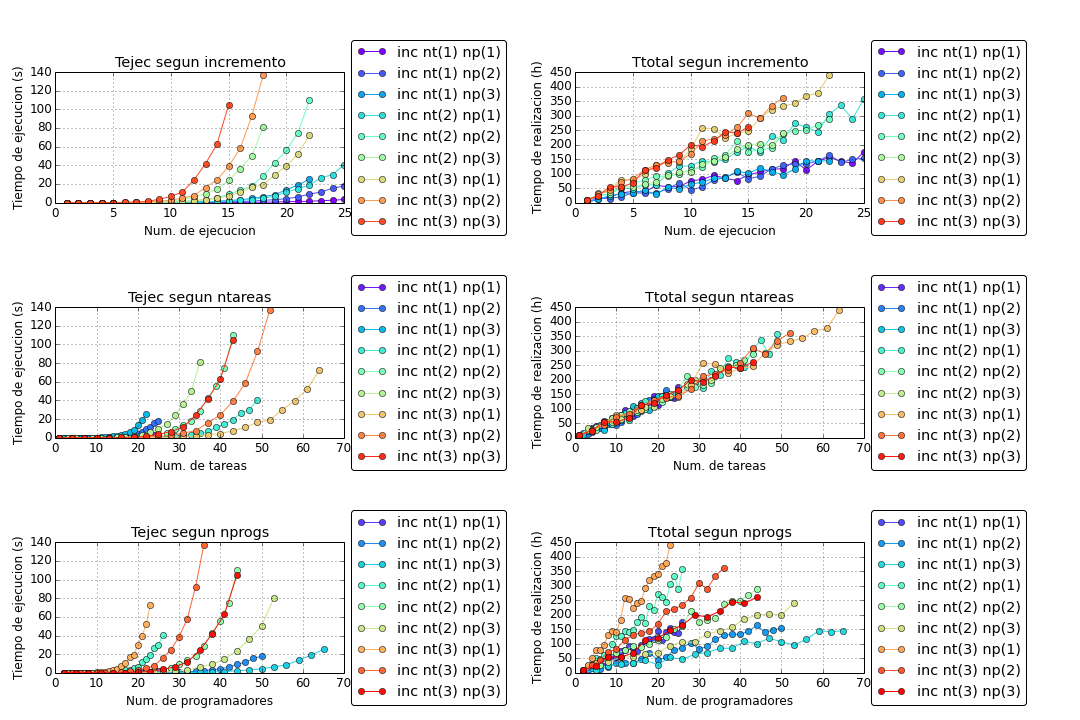
\includegraphics[height=13cm]{graph-2-1-2}
        \caption{Gráficos de los tiempos de ejecución para obtener las 
            soluciones y de los tiempos totales de desarrollo de estas en 
            función del tamaño de la entrada para la extensión 2.}
        \label{fig:extra-ext2}
    \end{figure}

\end{landscape}
}

En los gráficos de la mitad izquierda, correpondientes al tiempo de ejecución 
del \texttt{Fast Forward} para obtener la solución, se aprecia que para 
valores muy bajos la resolución es prácticamente instantánea y, a partir de 
un cierto tamaño, el tiempo de ejecución empieza a crecer de forma muy rápida 
(con los tamaños que hemos podido probar debido a las limitaciones del 
\textit{parser} del \texttt{Fast Forward} no podemos sacar conclusiones 
definitivas, pero podría tratarse de funciones polinómicas de un grado 
bastante alto, según el factor de ramificación). Esto se debe a que el 
planificador, en primera instancia, intenta encontrar una solución de forma 
rápida usando algoritmos de búsqueda local guiados por heurísticas genéricas, 
pero si no la encuentra luego procede con un algoritmo de búsqueda de tipo
\textit{best-first} que puede ser exhaustivo. Por lo tanto, para entradas 
muy pequeñas es probable que el planificador pueda hallar la respuesta con 
la primera búsqueda local pero esta ya no funcione a medida que la entrada 
crece. En este caso, como la búsqueda es prácticamente exhaustiva, el tiempo 
de ejecución depende esencialmente del factor de ramificación dado por las 
acciones del modelo.

En los gráficos de la derecha, en cambio, se representa la calidad de las 
soluciones obtenidas; es decir, la suma de las horas que los programadores 
invertirán para realizar todas las tareas asignadas en las soluciones 
obtenidas. Se aprecia claramente que, en todos los casos, este tiempo de 
resolución depende linealmente del tamaño de la entrada (básicamente del 
número de tareas). Parece muy razonable, teniendo en cuenta que los 
problemas se generan de forma aleatoria y homogénea, que el aumento del 
tiempo necesario para la realización de las tareas aumente proporcionalmente 
a la cantidad de estas (y, por lo tanto, en menor medida se aprecia en los 
gráficos una dependencia también del número de programadores, pero esto es 
porque se ha intentado mantener un cierto equilibrio entre el número de 
tareas y el número de programadores para comparar mejor la calidad de las 
soluciones). Es decir, el tiempo de resolución de las tareas depende 
linealmente del número de tareas, con una alta correlación, pero no depende 
prácticamente del número de programadores (siempre y cuando haya un número 
mínimo de programadores capaces de realizar las tareas siguiendo las 
restricciones del problema).

Se han realizado pruebas similares para todas las versiones del problema 
(las tablas y los gráficos resultantes están incluidos en los archivos 
adjuntos a este documento). El análisis de estos resultados se omite en este 
informe porque las tendencias que se aprecian en los gráficos son 
prácticamente las mismas.





\clearpage

